\chapter{Теоретическая часть}
\label{cha:ch_1}

\section{Физика звука}
Звук - это вибрация, которая распространяется через воздух (или воду).
Например, при прослушивании музыки с компьютера колонки производят вибрации,
которые распространяются по воздуху, пока не достигнут уха человека.

Вибрации можно смоделировать с помощью синусоидальных волн.

\subsection{Чистый тон}
Чистый тон - это тон синусоидальной формы волны. Характеристики синусоиды:
\begin{itemize}
    \item Частота: количество циклов в секунду. Единица измерения - Герц (Гц), например, 100 Гц = 100 циклов в секунду.
    \item Амплитуда (связана с громкостью звука): размер каждого цикла.
\end{itemize}

Эти характеристики расшифровываются человеческим ухом для формирования звука.
Человек может слышать чистые тоны от $20$ Гц до $20 000$ Гц,
и этот диапазон уменьшается с возрастом. Для сравнения, свет, который видит человек,
состоит из синусоид от $4 * 10^{14}$ Гц до $7.9 * 10^{14}$ Гц.

Человеческое восприятие громкости зависит от частоты чистого тона.
Например, чистый тон с амплитудой равной $10$ и частотой $30$ Гц будет тише,
чем чистый тон с амплитудой $10$ и частотой $1000$ Гц.
Человеческие уши воспринимают звук в соответствии с психоакустической моделью.

Чистых тонов в природе не существует, однако каждый звук в мире - это сумма
нескольких чистых тонов с разными амплитудами.

\subsection{Музыкальные ноты}
Ноты разделены на октавы. В большинстве западных стран октава представляет
собой набор из 8 нот (A, B, C, D, E, F, G в большинстве англоязычных
стран) со следующим свойством:
\begin{itemize}
    \item Частота ноты в октаве удваивается в следующей октаве.
    Например, частота А4 (А в 4-й октаве) на частоте 440 Гц в 2 раза
    превышает частоту А3 (А в 3-й октаве) на 220 Гц и в 4 раза больше
    частоты А2 (А во 2-й октаве) на 110 Гц.
\end{itemize}

% Для 4-й октавы ноты имеют следующую частоту:
% \begin{itemize}
%     \item C4 = 261.63 Гц
%     \item D4  = 293.67 Гц
%     \item E4 = 329.63 Гц
%     \item F4 = 349.23 Гц
%     \item G4 = 392 Гц
%     \item A4 = 440 Гц
%     \item B4 = 493.88 Гц
% \end{itemize}

Частотная чувствительность ушей логарифмическая. Это означает, что:
\begin{itemize}
    \item между 32.70 Гц и 61.74 Гц (1-я октава)
    \item или между 261.63 Гц и 466.16 Гц (4-я октава)
    \item или между 2 093 Гц и 3 951.07 Гц (7-я октава)
\end{itemize}

Человеческие уши распознают одинаковое количество нот.


\section{Техника акустического отпечатка}
Для того, чтобы эффективно хранить и искать аудиофайлы, нужно
найти какое-нибудь компактное представление, которое при этом будет
максимально правдоподобно их описывать.
Это представление называется акустическим отпечатком (фингерпринтом) аудиофайла.
Существует множество видов таких отпечатков, но большинство методов
находят представление аудиофайлов в виде вектора хешей.

Факторы эффективности:
\begin{enumerate}[label=\arabic*.]
    \item Хеши максимизируют произведение функций энтропии и точности:
    \begin{center}
        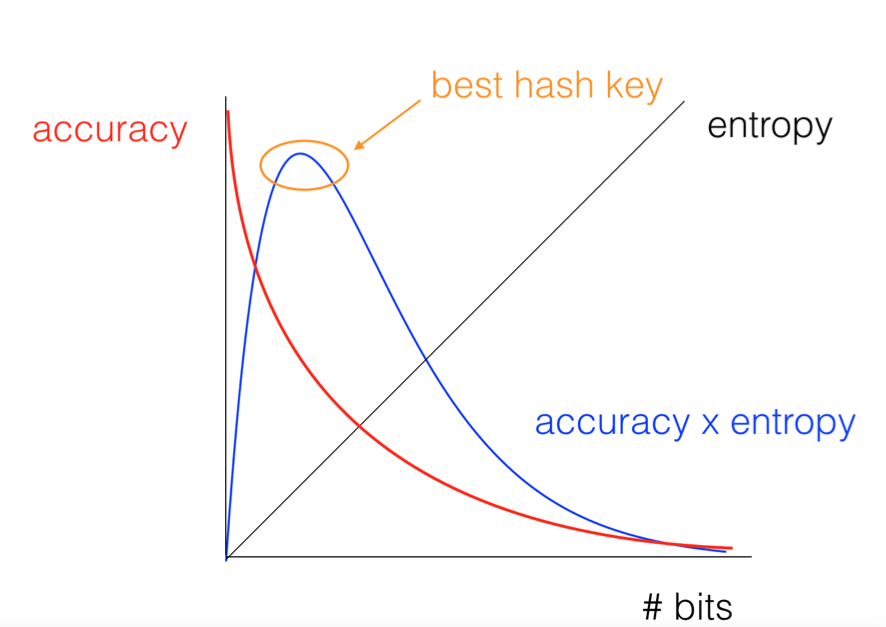
\includegraphics[scale=0.6]{inc/img/best_hp.png}
    \end{center}
    \item Биты хешей сбалансированы, декоррелированы и имеют высокую дисперсию
\end{enumerate}

\subsection{Общая идея}
Многие алгоритмы фингерпринтинга выглядят так:
\begin{enumerate}[label=\arabic*.]
    % \item Индексация:
    % \begin{enumerate}
        \item Посчитать спектрограмму аудиофайла
        \item Применить на ней какую-либо оконную функцию (спектрально-временные фильтры)
        \item Конвертировать результат в вектор хешей
    %     \item Посчитать обратный индекс вида:
    %     $$hash \to [... \{song\_id,\ offset\} ... ]$$, где $offset$ -- это
    %     номер временного диапазона аудиофайла, соответствующего $song\_id$,
    %     в котором встречается $hash$.
    % \end{enumerate}
    % \item Поиск:
    % \begin{enumerate}
    %     \item Посчитать акустический отпечаток запроса
    %     \item Поскольку
    % \end{enumerate}
\end{enumerate}

\section{Метод хешпринтов}
Этот метод предложен в \cite{tsai}. Он, как и многие другие, находит представление
аудиофайла в виде вектора хешей.

Метод отличается следующими характеристиками:
\begin{enumerate}[label=\arabic*.]
    \item Обучение без учителя
    \item Высокая адаптивность к данным
    \item Независимость от силы сигнала (громкости звука)
\end{enumerate}

Самой важной отличительной чертой метода является обучение без учителя.
Такие методы, как, например, Chromaprint, описанный в \cite{chromaprint}, используют
заранее подготовленные спектрально-временные фильтры.
Метод хешпринтов находит эти фильтры непосредственно при индексации, что позволяет
ему учитывать специфику данных.
\begin{figure}
    \begin{center}
        
\includegraphics[scale=0.3]{inc/img/chroma.png}
        \caption{Фильтры, используемые Chromaprint}
    \end{center}
\end{figure}

\subsection{Алгоритм вычисления хешпринта}
Для вычисления хешпринта, содержащего $N$ бит, нужно проделать следующее:
\begin{enumerate}[label=\arabic*.]
    \item Посчитать спектрограмму.\\
    Результат этапа: матрица $Spectrogram \in \mathbb{R}^{B \times n}$, где $B$ -- количество частотных диапазонов,
    $n$ -- количество временных диапазонов.
    \item Собрать контекстные фреймы полученной спектрограммы.
    Фреймы рассчитываются следующим образом:
    $$frame_i = V_{i-w}...V_{i+w}$$, где $V_i$ -- столбец спектрограммы, $w$ -- количество столбцов контекста.\\
    Результат этапа: матрица $Frames \in \mathbb{R}^{Bw \times n}$
    \item Применить к фреймам спектрально-временные фильтры. Фильтры представляют собой
    $N \times Bw$ матрицу и расситываются c помощью алгоритма обучения без учителя
    путем решения задачи оптимизации.\\
    Результат этапа: матрица признаков $Features \in \mathbb{R}^{N \times n}$.
    \item Посчитать дельту -- изменение признаков в течение промежутка $T$.
    Дельта рассчитывается по формуле:
    $$\Delta_i = feature_i - feature_{i+T}$$
    \item Наложить функцию порога и упаковать признаки в хешпринты:
    $$hashprint_i = intN(\Delta_i > 0)$$
\end{enumerate}

\subsection{Вычисление спектрально-временных фильтров}
Фильтры подбираются таким образом, чтобы признаки, полученные при их наложении,
имели максимальную дисперсию и в то же время были декоррелированы.\\
Для этого можно применить метод главных компонент (PCA):
\begin{enumerate}[label=\arabic*.]
    \item Посчитать ковариационные матрицы для всех матриц фреймов
    и просуммировать их.\\
    Результат этапа: матрица $CovarianceMatrix \in \mathbb{R}^{Bw \times Bw}$
    \item Найти $N$ собственных векторов с максимальными собственными значениями.\\
    Результат этапа: матрица $Filters \in \mathbb{R}^{N \times Bw}$
\end{enumerate}

\subsection{Специфика задачи идентификации живых отрывков}
Поскольку речь идет о нечетком поиске, то мы хотим учесть как можно
больше нюансов (признаков) сигнала. Поэтому будем представлять аудиофайлы в виде
64-битных хешпринтов. Также в качестве спектрограммы возьмем CQT спектрограмму -
она хороша тем, что ее частотные диапазоны можно подобрать таким образом, что они будут
соответствовать конкретным нотам.
Из-за того что мы имеем дело с пространством довольно большой размерности, мы не можем
использовать обратный индекс, поэтому поиск будет выглядеть примерно так:
\begin{enumerate}[label=\arabic*.]
    \item Для каждого оригинала из базы: прикладываем к нему отрывок и ищем такой отступ, чтобы сумма расстояний
    Хемминга между соответствующими хешпринтами была минимальной.
    \begin{center}
        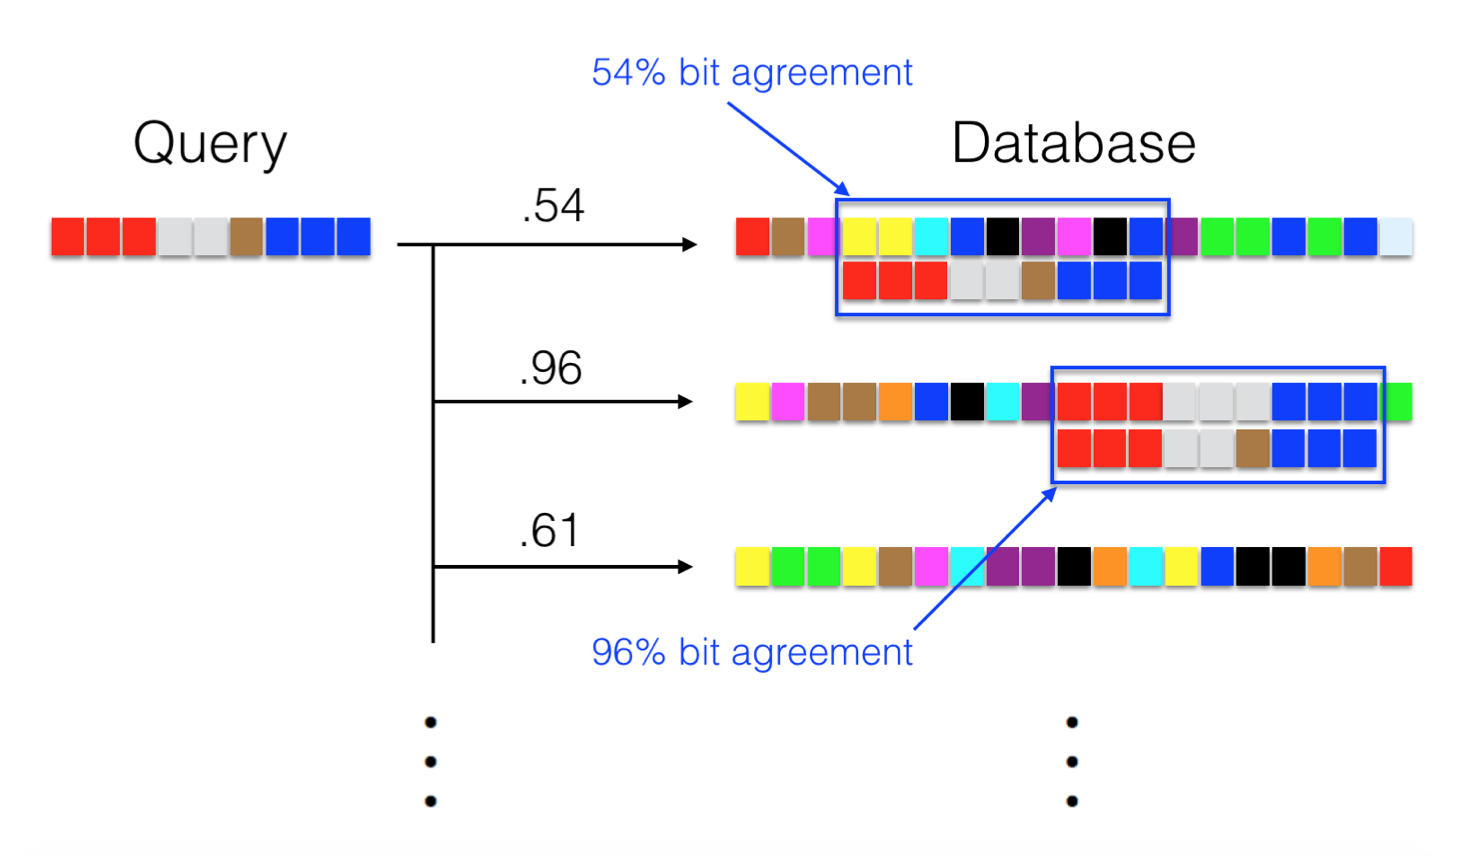
\includegraphics[scale=0.5]{inc/img/query.png}
    \end{center}
    \item Собираем результаты, сортируем и возвращаем top-N
\end{enumerate}
